\documentclass[1p]{elsarticle_modified}
%\bibliographystyle{elsarticle-num}

%\usepackage[colorlinks]{hyperref}
%\usepackage{abbrmath_seonhwa} %\Abb, \Ascr, \Acal ,\Abf, \Afrak
\usepackage{amsfonts}
\usepackage{amssymb}
\usepackage{amsmath}
\usepackage{amsthm}
\usepackage{scalefnt}
\usepackage{amsbsy}
\usepackage{kotex}
\usepackage{caption}
\usepackage{subfig}
\usepackage{color}
\usepackage{graphicx}
\usepackage{xcolor} %% white, black, red, green, blue, cyan, magenta, yellow
\usepackage{float}
\usepackage{setspace}
\usepackage{hyperref}

\usepackage{tikz}
\usetikzlibrary{arrows}

\usepackage{multirow}
\usepackage{array} % fixed length table
\usepackage{hhline}

%%%%%%%%%%%%%%%%%%%%%
\makeatletter
\renewcommand*\env@matrix[1][\arraystretch]{%
	\edef\arraystretch{#1}%
	\hskip -\arraycolsep
	\let\@ifnextchar\new@ifnextchar
	\array{*\c@MaxMatrixCols c}}
\makeatother %https://tex.stackexchange.com/questions/14071/how-can-i-increase-the-line-spacing-in-a-matrix
%%%%%%%%%%%%%%%

\usepackage[normalem]{ulem}

\newcommand{\msout}[1]{\ifmmode\text{\sout{\ensuremath{#1}}}\else\sout{#1}\fi}
%SOURCE: \msout is \stkout macro in https://tex.stackexchange.com/questions/20609/strikeout-in-math-mode

\newcommand{\cancel}[1]{
	\ifmmode
	{\color{red}\msout{#1}}
	\else
	{\color{red}\sout{#1}}
	\fi
}

\newcommand{\add}[1]{
	{\color{blue}\uwave{#1}}
}

\newcommand{\replace}[2]{
	\ifmmode
	{\color{red}\msout{#1}}{\color{blue}\uwave{#2}}
	\else
	{\color{red}\sout{#1}}{\color{blue}\uwave{#2}}
	\fi
}

\newcommand{\Sol}{\mathcal{S}} %segment
\newcommand{\D}{D} %diagram
\newcommand{\A}{\mathcal{A}} %arc


%%%%%%%%%%%%%%%%%%%%%%%%%%%%%5 test

\def\sl{\operatorname{\textup{SL}}(2,\Cbb)}
\def\psl{\operatorname{\textup{PSL}}(2,\Cbb)}
\def\quan{\mkern 1mu \triangleright \mkern 1mu}

\theoremstyle{definition}
\newtheorem{thm}{Theorem}[section]
\newtheorem{prop}[thm]{Proposition}
\newtheorem{lem}[thm]{Lemma}
\newtheorem{ques}[thm]{Question}
\newtheorem{cor}[thm]{Corollary}
\newtheorem{defn}[thm]{Definition}
\newtheorem{exam}[thm]{Example}
\newtheorem{rmk}[thm]{Remark}
\newtheorem{alg}[thm]{Algorithm}

\newcommand{\I}{\sqrt{-1}}
\begin{document}

%\begin{frontmatter}
%
%\title{Boundary parabolic representations of knots up to 8 crossings}
%
%%% Group authors per affiliation:
%\author{Yunhi Cho} 
%\address{Department of Mathematics, University of Seoul, Seoul, Korea}
%\ead{yhcho@uos.ac.kr}
%
%
%\author{Seonhwa Kim} %\fnref{s_kim}}
%\address{Center for Geometry and Physics, Institute for Basic Science, Pohang, 37673, Korea}
%\ead{ryeona17@ibs.re.kr}
%
%\author{Hyuk Kim}
%\address{Department of Mathematical Sciences, Seoul National University, Seoul 08826, Korea}
%\ead{hyukkim@snu.ac.kr}
%
%\author{Seokbeom Yoon}
%\address{Department of Mathematical Sciences, Seoul National University, Seoul, 08826,  Korea}
%\ead{sbyoon15@snu.ac.kr}
%
%\begin{abstract}
%We find all boundary parabolic representation of knots up to 8 crossings.
%
%\end{abstract}
%\begin{keyword}
%    \MSC[2010] 57M25 
%\end{keyword}
%
%\end{frontmatter}

%\linenumbers
%\tableofcontents
%
\newcommand\colored[1]{\textcolor{white}{\rule[-0.35ex]{0.8em}{1.4ex}}\kern-0.8em\color{red} #1}%
%\newcommand\colored[1]{\textcolor{white}{ #1}\kern-2.17ex	\textcolor{white}{ #1}\kern-1.81ex	\textcolor{white}{ #1}\kern-2.15ex\color{red}#1	}

{\Large $\underline{12a_{0277}~(K12a_{0277})}$}

\setlength{\tabcolsep}{10pt}
\renewcommand{\arraystretch}{1.6}
\vspace{1cm}\begin{tabular}{m{100pt}>{\centering\arraybackslash}m{274pt}}
\multirow{5}{120pt}{
	\centering
	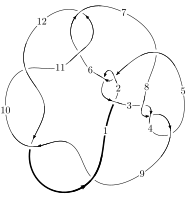
\includegraphics[width=112pt]{../../../GIT/diagram.site/Diagrams/png/1078_12a_0277.png}\\
\ \ \ A knot diagram\footnotemark}&
\allowdisplaybreaks
\textbf{Linearized knot diagam} \\
\cline{2-2}
 &
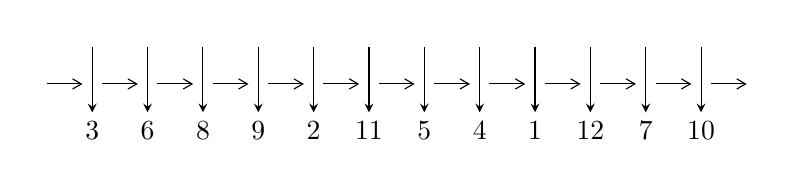
\begin{tikzpicture}[x=20pt, y=17pt]
	% nodes
	\node (C0) at (0, 0) {};
	\node (C1) at (1, 0) {};
	\node (C1U) at (1, +1) {};
	\node (C1D) at (1, -1) {3};

	\node (C2) at (2, 0) {};
	\node (C2U) at (2, +1) {};
	\node (C2D) at (2, -1) {6};

	\node (C3) at (3, 0) {};
	\node (C3U) at (3, +1) {};
	\node (C3D) at (3, -1) {8};

	\node (C4) at (4, 0) {};
	\node (C4U) at (4, +1) {};
	\node (C4D) at (4, -1) {9};

	\node (C5) at (5, 0) {};
	\node (C5U) at (5, +1) {};
	\node (C5D) at (5, -1) {2};

	\node (C6) at (6, 0) {};
	\node (C6U) at (6, +1) {};
	\node (C6D) at (6, -1) {11};

	\node (C7) at (7, 0) {};
	\node (C7U) at (7, +1) {};
	\node (C7D) at (7, -1) {5};

	\node (C8) at (8, 0) {};
	\node (C8U) at (8, +1) {};
	\node (C8D) at (8, -1) {4};

	\node (C9) at (9, 0) {};
	\node (C9U) at (9, +1) {};
	\node (C9D) at (9, -1) {1};

	\node (C10) at (10, 0) {};
	\node (C10U) at (10, +1) {};
	\node (C10D) at (10, -1) {12};

	\node (C11) at (11, 0) {};
	\node (C11U) at (11, +1) {};
	\node (C11D) at (11, -1) {7};

	\node (C12) at (12, 0) {};
	\node (C12U) at (12, +1) {};
	\node (C12D) at (12, -1) {10};
	\node (C13) at (13, 0) {};

	% arrows
	\draw[->,>={angle 60}]
	(C0) edge (C1) (C1) edge (C2) (C2) edge (C3) (C3) edge (C4) (C4) edge (C5) (C5) edge (C6) (C6) edge (C7) (C7) edge (C8) (C8) edge (C9) (C9) edge (C10) (C10) edge (C11) (C11) edge (C12) (C12) edge (C13) ;	\draw[->,>=stealth]
	(C1U) edge (C1D) (C2U) edge (C2D) (C3U) edge (C3D) (C4U) edge (C4D) (C5U) edge (C5D) (C6U) edge (C6D) (C7U) edge (C7D) (C8U) edge (C8D) (C9U) edge (C9D) (C10U) edge (C10D) (C11U) edge (C11D) (C12U) edge (C12D) ;
	\end{tikzpicture} \\
\hhline{~~} \\& 
\textbf{Solving Sequence} \\ \cline{2-2} 
 &
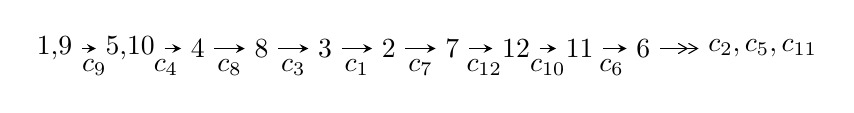
\begin{tikzpicture}[x=23pt, y=7pt]
	% node
	\node (A0) at (-1/8, 0) {1,9};
	\node (A1) at (17/16, 0) {5,10};
	\node (A2) at (17/8, 0) {4};
	\node (A3) at (25/8, 0) {8};
	\node (A4) at (33/8, 0) {3};
	\node (A5) at (41/8, 0) {2};
	\node (A6) at (49/8, 0) {7};
	\node (A7) at (57/8, 0) {12};
	\node (A8) at (65/8, 0) {11};
	\node (A9) at (73/8, 0) {6};
	\node (C1) at (1/2, -1) {$c_{9}$};
	\node (C2) at (13/8, -1) {$c_{4}$};
	\node (C3) at (21/8, -1) {$c_{8}$};
	\node (C4) at (29/8, -1) {$c_{3}$};
	\node (C5) at (37/8, -1) {$c_{1}$};
	\node (C6) at (45/8, -1) {$c_{7}$};
	\node (C7) at (53/8, -1) {$c_{12}$};
	\node (C8) at (61/8, -1) {$c_{10}$};
	\node (C9) at (69/8, -1) {$c_{6}$};
	\node (A10) at (11, 0) {$c_{2},c_{5},c_{11}$};

	% edge
	\draw[->,>=stealth]	
	(A0) edge (A1) (A1) edge (A2) (A2) edge (A3) (A3) edge (A4) (A4) edge (A5) (A5) edge (A6) (A6) edge (A7) (A7) edge (A8) (A8) edge (A9) ;
	\draw[->>,>={angle 60}]	
	(A9) edge (A10);
\end{tikzpicture} \\ 

\end{tabular} \\

\footnotetext{
The image of knot diagram is generated by the software ``\textbf{Draw programme}" developed by Andrew Bartholomew(\url{http://www.layer8.co.uk/maths/draw/index.htm\#Running-draw}), where we modified some parts for our purpose(\url{https://github.com/CATsTAILs/LinksPainter}).
}\phantom \\ \newline 
\centering \textbf{Ideals for irreducible components\footnotemark of $X_{\text{par}}$} 
 
\begin{align*}
I^u_{1}&=\langle 
-4.72311\times10^{64} u^{79}+9.32849\times10^{65} u^{78}+\cdots+1.78584\times10^{64} b+1.98266\times10^{65},\\
\phantom{I^u_{1}}&\phantom{= \langle  }1.08221\times10^{65} u^{79}-2.14479\times10^{66} u^{78}+\cdots+1.78584\times10^{64} a-3.42835\times10^{65},\;u^{80}-20 u^{79}+\cdots-18 u+1\rangle \\
I^u_{2}&=\langle 
b^2-2,\;- u^2+a+u-2,\;u^3- u^2+2 u-1\rangle \\
I^u_{3}&=\langle 
b,\;u^2+a- u+2,\;u^3- u^2+2 u-1\rangle \\
\\
\end{align*}
\raggedright * 3 irreducible components of $\dim_{\mathbb{C}}=0$, with total 89 representations.\\
\footnotetext{All coefficients of polynomials are rational numbers. But the coefficients are sometimes approximated in decimal forms when there is not enough margin.}
\newpage
\renewcommand{\arraystretch}{1}
\centering \section*{I. $I^u_{1}= \langle -4.72\times10^{64} u^{79}+9.33\times10^{65} u^{78}+\cdots+1.79\times10^{64} b+1.98\times10^{65},\;1.08\times10^{65} u^{79}-2.14\times10^{66} u^{78}+\cdots+1.79\times10^{64} a-3.43\times10^{65},\;u^{80}-20 u^{79}+\cdots-18 u+1 \rangle$}
\flushleft \textbf{(i) Arc colorings}\\
\begin{tabular}{m{7pt} m{180pt} m{7pt} m{180pt} }
\flushright $a_{1}=$&$\begin{pmatrix}0\\u\end{pmatrix}$ \\
\flushright $a_{9}=$&$\begin{pmatrix}1\\0\end{pmatrix}$ \\
\flushright $a_{5}=$&$\begin{pmatrix}-6.05997 u^{79}+120.100 u^{78}+\cdots-283.148 u+19.1974\\2.64476 u^{79}-52.2359 u^{78}+\cdots+160.871 u-11.1021\end{pmatrix}$ \\
\flushright $a_{10}=$&$\begin{pmatrix}1\\u^2\end{pmatrix}$ \\
\flushright $a_{4}=$&$\begin{pmatrix}-3.41521 u^{79}+67.8640 u^{78}+\cdots-122.277 u+8.09533\\2.64476 u^{79}-52.2359 u^{78}+\cdots+160.871 u-11.1021\end{pmatrix}$ \\
\flushright $a_{8}=$&$\begin{pmatrix}2.78759 u^{79}-55.0401 u^{78}+\cdots+4.23430 u+2.44867\\-2.71435 u^{79}+53.7245 u^{78}+\cdots-169.151 u+11.1549\end{pmatrix}$ \\
\flushright $a_{3}=$&$\begin{pmatrix}3.75953 u^{79}-74.3293 u^{78}+\cdots+112.373 u-6.62197\\-1.90562 u^{79}+37.5370 u^{78}+\cdots-107.936 u+6.96219\end{pmatrix}$ \\
\flushright $a_{2}=$&$\begin{pmatrix}-3.45746 u^{79}+68.4432 u^{78}+\cdots-98.6276 u+5.02931\\1.66130 u^{79}-32.7533 u^{78}+\cdots+100.748 u-6.43094\end{pmatrix}$ \\
\flushright $a_{7}=$&$\begin{pmatrix}-4.58743 u^{79}+90.5934 u^{78}+\cdots-281.163 u+21.8214\\0.879640 u^{79}-17.2874 u^{78}+\cdots+40.9055 u-3.15319\end{pmatrix}$ \\
\flushright $a_{12}=$&$\begin{pmatrix}u\\u^3+u\end{pmatrix}$ \\
\flushright $a_{11}=$&$\begin{pmatrix}u^2+1\\u^4+2 u^2\end{pmatrix}$ \\
\flushright $a_{6}=$&$\begin{pmatrix}-3.15319 u^{79}+62.1841 u^{78}+\cdots-201.223 u+15.8519\\0.849761 u^{79}-16.8147 u^{78}+\cdots+48.0720 u-3.70779\end{pmatrix}$\\&\end{tabular}
\flushleft \textbf{(ii) Obstruction class $= -1$}\\~\\
\flushleft \textbf{(iii) Cusp Shapes $= 5.49769 u^{79}-108.641 u^{78}+\cdots+342.310 u-39.1178$}\\~\\
\newpage\renewcommand{\arraystretch}{1}
\flushleft \textbf{(iv) u-Polynomials at the component}\newline \\
\begin{tabular}{m{50pt}|m{274pt}}
Crossings & \hspace{64pt}u-Polynomials at each crossing \\
\hline $$\begin{aligned}c_{1}\end{aligned}$$&$\begin{aligned}
&u^{80}+38 u^{79}+\cdots+15621 u+529
\end{aligned}$\\
\hline $$\begin{aligned}c_{2},c_{5}\end{aligned}$$&$\begin{aligned}
&u^{80}+4 u^{79}+\cdots-163 u-23
\end{aligned}$\\
\hline $$\begin{aligned}c_{3},c_{4},c_{8}\end{aligned}$$&$\begin{aligned}
&u^{80}+u^{79}+\cdots-8 u-8
\end{aligned}$\\
\hline $$\begin{aligned}c_{6},c_{11}\end{aligned}$$&$\begin{aligned}
&u^{80}-2 u^{79}+\cdots-4 u-1
\end{aligned}$\\
\hline $$\begin{aligned}c_{7}\end{aligned}$$&$\begin{aligned}
&u^{80}-3 u^{79}+\cdots+5400 u+1000
\end{aligned}$\\
\hline $$\begin{aligned}c_{9},c_{10},c_{12}\end{aligned}$$&$\begin{aligned}
&u^{80}+20 u^{79}+\cdots+18 u+1
\end{aligned}$\\
\hline
\end{tabular}\\~\\
\newpage\renewcommand{\arraystretch}{1}
\flushleft \textbf{(v) Riley Polynomials at the component}\newline \\
\begin{tabular}{m{50pt}|m{274pt}}
Crossings & \hspace{64pt}Riley Polynomials at each crossing \\
\hline $$\begin{aligned}c_{1}\end{aligned}$$&$\begin{aligned}
&y^{80}+18 y^{79}+\cdots-20758597 y+279841
\end{aligned}$\\
\hline $$\begin{aligned}c_{2},c_{5}\end{aligned}$$&$\begin{aligned}
&y^{80}-38 y^{79}+\cdots-15621 y+529
\end{aligned}$\\
\hline $$\begin{aligned}c_{3},c_{4},c_{8}\end{aligned}$$&$\begin{aligned}
&y^{80}-73 y^{79}+\cdots+576 y+64
\end{aligned}$\\
\hline $$\begin{aligned}c_{6},c_{11}\end{aligned}$$&$\begin{aligned}
&y^{80}-20 y^{79}+\cdots-18 y+1
\end{aligned}$\\
\hline $$\begin{aligned}c_{7}\end{aligned}$$&$\begin{aligned}
&y^{80}+11 y^{79}+\cdots+9560000 y+1000000
\end{aligned}$\\
\hline $$\begin{aligned}c_{9},c_{10},c_{12}\end{aligned}$$&$\begin{aligned}
&y^{80}+84 y^{79}+\cdots+86 y+1
\end{aligned}$\\
\hline
\end{tabular}\\~\\
\newpage\flushleft \textbf{(vi) Complex Volumes and Cusp Shapes}
$$\begin{array}{c|c|c}  
\text{Solutions to }I^u_{1}& \I (\text{vol} + \sqrt{-1}CS) & \text{Cusp shape}\\
 \hline 
\begin{aligned}
u &= \phantom{-}0.514598 + 0.797614 I \\
a &= -0.182271 + 0.963044 I \\
b &= -0.166867 - 0.621031 I\end{aligned}
 & \phantom{-}1.34935 - 2.65440 I & \phantom{-0.000000 } 0 \\ \hline\begin{aligned}
u &= \phantom{-}0.514598 - 0.797614 I \\
a &= -0.182271 - 0.963044 I \\
b &= -0.166867 + 0.621031 I\end{aligned}
 & \phantom{-}1.34935 + 2.65440 I & \phantom{-0.000000 } 0 \\ \hline\begin{aligned}
u &= \phantom{-}0.930722 + 0.185711 I \\
a &= \phantom{-}0.009280 + 0.280137 I \\
b &= \phantom{-}0.181905 - 0.585150 I\end{aligned}
 & -2.18248 + 1.71695 I & \phantom{-0.000000 } 0 \\ \hline\begin{aligned}
u &= \phantom{-}0.930722 - 0.185711 I \\
a &= \phantom{-}0.009280 - 0.280137 I \\
b &= \phantom{-}0.181905 + 0.585150 I\end{aligned}
 & -2.18248 - 1.71695 I & \phantom{-0.000000 } 0 \\ \hline\begin{aligned}
u &= \phantom{-}0.919274 + 0.137908 I \\
a &= \phantom{-}0.747010 + 0.189533 I \\
b &= \phantom{-}1.288870 - 0.122433 I\end{aligned}
 & -5.31070 + 0.42006 I & \phantom{-0.000000 } 0 \\ \hline\begin{aligned}
u &= \phantom{-}0.919274 - 0.137908 I \\
a &= \phantom{-}0.747010 - 0.189533 I \\
b &= \phantom{-}1.288870 + 0.122433 I\end{aligned}
 & -5.31070 - 0.42006 I & \phantom{-0.000000 } 0 \\ \hline\begin{aligned}
u &= \phantom{-}1.030150 + 0.302517 I \\
a &= -0.848263 - 0.262462 I \\
b &= -1.366380 + 0.243133 I\end{aligned}
 & -7.10040 + 4.78774 I & \phantom{-0.000000 } 0 \\ \hline\begin{aligned}
u &= \phantom{-}1.030150 - 0.302517 I \\
a &= -0.848263 + 0.262462 I \\
b &= -1.366380 - 0.243133 I\end{aligned}
 & -7.10040 - 4.78774 I & \phantom{-0.000000 } 0 \\ \hline\begin{aligned}
u &= \phantom{-}0.609392 + 0.691381 I \\
a &= \phantom{-}0.204257 + 0.417749 I \\
b &= \phantom{-}0.629301 - 0.385404 I\end{aligned}
 & -1.82971 - 3.50991 I & \phantom{-0.000000 } 0 \\ \hline\begin{aligned}
u &= \phantom{-}0.609392 - 0.691381 I \\
a &= \phantom{-}0.204257 - 0.417749 I \\
b &= \phantom{-}0.629301 + 0.385404 I\end{aligned}
 & -1.82971 + 3.50991 I & \phantom{-0.000000 } 0\\
 \hline 
 \end{array}$$\newpage$$\begin{array}{c|c|c}  
\text{Solutions to }I^u_{1}& \I (\text{vol} + \sqrt{-1}CS) & \text{Cusp shape}\\
 \hline 
\begin{aligned}
u &= \phantom{-}0.755355 + 0.786820 I \\
a &= \phantom{-}0.28069 - 1.41735 I \\
b &= \phantom{-}1.347050 + 0.254095 I\end{aligned}
 & -3.40751 - 5.86732 I & \phantom{-0.000000 } 0 \\ \hline\begin{aligned}
u &= \phantom{-}0.755355 - 0.786820 I \\
a &= \phantom{-}0.28069 + 1.41735 I \\
b &= \phantom{-}1.347050 - 0.254095 I\end{aligned}
 & -3.40751 + 5.86732 I & \phantom{-0.000000 } 0 \\ \hline\begin{aligned}
u &= \phantom{-}0.788627 + 0.790526 I \\
a &= \phantom{-}0.437053 - 0.837105 I \\
b &= \phantom{-}0.269993 + 0.717932 I\end{aligned}
 & -0.40460 - 7.35219 I & \phantom{-0.000000 } 0 \\ \hline\begin{aligned}
u &= \phantom{-}0.788627 - 0.790526 I \\
a &= \phantom{-}0.437053 + 0.837105 I \\
b &= \phantom{-}0.269993 - 0.717932 I\end{aligned}
 & -0.40460 + 7.35219 I & \phantom{-0.000000 } 0 \\ \hline\begin{aligned}
u &= \phantom{-}0.684330 + 0.553457 I \\
a &= \phantom{-}0.01541 + 2.37497 I \\
b &= -1.388830 - 0.162566 I\end{aligned}
 & -8.24545 - 2.75079 I & \phantom{-0.000000 } 0 \\ \hline\begin{aligned}
u &= \phantom{-}0.684330 - 0.553457 I \\
a &= \phantom{-}0.01541 - 2.37497 I \\
b &= -1.388830 + 0.162566 I\end{aligned}
 & -8.24545 + 2.75079 I & \phantom{-0.000000 } 0 \\ \hline\begin{aligned}
u &= -0.127842 + 0.864691 I \\
a &= -0.255160 + 0.396206 I \\
b &= \phantom{-}1.260690 + 0.244422 I\end{aligned}
 & -1.23948 - 4.76112 I & \phantom{-0.000000 } 0 \\ \hline\begin{aligned}
u &= -0.127842 - 0.864691 I \\
a &= -0.255160 - 0.396206 I \\
b &= \phantom{-}1.260690 - 0.244422 I\end{aligned}
 & -1.23948 + 4.76112 I & \phantom{-0.000000 } 0 \\ \hline\begin{aligned}
u &= \phantom{-}0.419774 + 1.097820 I \\
a &= \phantom{-}0.077772 - 0.334119 I \\
b &= \phantom{-}1.194940 + 0.059585 I\end{aligned}
 & -1.55006 - 4.38158 I & \phantom{-0.000000 } 0 \\ \hline\begin{aligned}
u &= \phantom{-}0.419774 - 1.097820 I \\
a &= \phantom{-}0.077772 + 0.334119 I \\
b &= \phantom{-}1.194940 - 0.059585 I\end{aligned}
 & -1.55006 + 4.38158 I & \phantom{-0.000000 } 0\\
 \hline 
 \end{array}$$\newpage$$\begin{array}{c|c|c}  
\text{Solutions to }I^u_{1}& \I (\text{vol} + \sqrt{-1}CS) & \text{Cusp shape}\\
 \hline 
\begin{aligned}
u &= \phantom{-}0.680437 + 0.465530 I \\
a &= -0.917464 - 0.679063 I \\
b &= -1.47224 + 0.10694 I\end{aligned}
 & -8.51159 - 1.83203 I & \phantom{-0.000000 } 0 \\ \hline\begin{aligned}
u &= \phantom{-}0.680437 - 0.465530 I \\
a &= -0.917464 + 0.679063 I \\
b &= -1.47224 - 0.10694 I\end{aligned}
 & -8.51159 + 1.83203 I & \phantom{-0.000000 } 0 \\ \hline\begin{aligned}
u &= \phantom{-}0.894405 + 0.764372 I \\
a &= -0.61624 + 1.42654 I \\
b &= -1.40800 - 0.29107 I\end{aligned}
 & -5.74546 - 11.03100 I & \phantom{-0.000000 } 0 \\ \hline\begin{aligned}
u &= \phantom{-}0.894405 - 0.764372 I \\
a &= -0.61624 - 1.42654 I \\
b &= -1.40800 + 0.29107 I\end{aligned}
 & -5.74546 + 11.03100 I & \phantom{-0.000000 } 0 \\ \hline\begin{aligned}
u &= \phantom{-}0.289262 + 1.239150 I \\
a &= -0.045610 + 0.413852 I \\
b &= \phantom{-}0.023350 - 0.410951 I\end{aligned}
 & \phantom{-}1.97481 - 2.69073 I & \phantom{-0.000000 } 0 \\ \hline\begin{aligned}
u &= \phantom{-}0.289262 - 1.239150 I \\
a &= -0.045610 - 0.413852 I \\
b &= \phantom{-}0.023350 + 0.410951 I\end{aligned}
 & \phantom{-}1.97481 + 2.69073 I & \phantom{-0.000000 } 0 \\ \hline\begin{aligned}
u &= \phantom{-}0.590617 + 0.310506 I \\
a &= \phantom{-}0.96087 - 1.72410 I \\
b &= \phantom{-}0.255679 + 0.386530 I\end{aligned}
 & -2.98638 - 0.61275 I & \phantom{-0.000000 } 0 \\ \hline\begin{aligned}
u &= \phantom{-}0.590617 - 0.310506 I \\
a &= \phantom{-}0.96087 + 1.72410 I \\
b &= \phantom{-}0.255679 - 0.386530 I\end{aligned}
 & -2.98638 + 0.61275 I & \phantom{-0.000000 } 0 \\ \hline\begin{aligned}
u &= \phantom{-}0.454841 + 1.317990 I \\
a &= -0.1307020 + 0.0215197 I \\
b &= -1.299560 + 0.177427 I\end{aligned}
 & -2.13245 - 0.48191 I & \phantom{-0.000000 } 0 \\ \hline\begin{aligned}
u &= \phantom{-}0.454841 - 1.317990 I \\
a &= -0.1307020 - 0.0215197 I \\
b &= -1.299560 - 0.177427 I\end{aligned}
 & -2.13245 + 0.48191 I & \phantom{-0.000000 } 0\\
 \hline 
 \end{array}$$\newpage$$\begin{array}{c|c|c}  
\text{Solutions to }I^u_{1}& \I (\text{vol} + \sqrt{-1}CS) & \text{Cusp shape}\\
 \hline 
\begin{aligned}
u &= -0.181005 + 0.568134 I \\
a &= \phantom{-}0.897771 + 0.786811 I \\
b &= \phantom{-}0.002312 - 0.687422 I\end{aligned}
 & \phantom{-}2.60603 - 1.37683 I & \phantom{-0.000000 } 0 \\ \hline\begin{aligned}
u &= -0.181005 - 0.568134 I \\
a &= \phantom{-}0.897771 - 0.786811 I \\
b &= \phantom{-}0.002312 + 0.687422 I\end{aligned}
 & \phantom{-}2.60603 + 1.37683 I & \phantom{-0.000000 } 0 \\ \hline\begin{aligned}
u &= -0.134787 + 0.567278 I \\
a &= \phantom{-}0.180641 - 1.107910 I \\
b &= -1.039780 - 0.137065 I\end{aligned}
 & -0.586277 - 0.026228 I & \phantom{-0.000000 } 0 \\ \hline\begin{aligned}
u &= -0.134787 - 0.567278 I \\
a &= \phantom{-}0.180641 + 1.107910 I \\
b &= -1.039780 + 0.137065 I\end{aligned}
 & -0.586277 + 0.026228 I & \phantom{-0.000000 } 0 \\ \hline\begin{aligned}
u &= \phantom{-}0.06859 + 1.42466 I \\
a &= \phantom{-}0.0103422 + 0.0743670 I \\
b &= \phantom{-}1.53685 + 0.05092 I\end{aligned}
 & -1.92343 - 1.06909 I & \phantom{-0.000000 } 0 \\ \hline\begin{aligned}
u &= \phantom{-}0.06859 - 1.42466 I \\
a &= \phantom{-}0.0103422 - 0.0743670 I \\
b &= \phantom{-}1.53685 - 0.05092 I\end{aligned}
 & -1.92343 + 1.06909 I & \phantom{-0.000000 } 0 \\ \hline\begin{aligned}
u &= \phantom{-}0.02099 + 1.43824 I \\
a &= -1.27488 + 1.90471 I \\
b &= \phantom{-}1.284890 - 0.223646 I\end{aligned}
 & -1.128470 - 0.060432 I & \phantom{-0.000000 } 0 \\ \hline\begin{aligned}
u &= \phantom{-}0.02099 - 1.43824 I \\
a &= -1.27488 - 1.90471 I \\
b &= \phantom{-}1.284890 + 0.223646 I\end{aligned}
 & -1.128470 + 0.060432 I & \phantom{-0.000000 } 0 \\ \hline\begin{aligned}
u &= -0.13847 + 1.45741 I \\
a &= -0.22590 + 1.82988 I \\
b &= \phantom{-}1.42465 - 0.34186 I\end{aligned}
 & \phantom{-}2.61988 + 9.27844 I & \phantom{-0.000000 } 0 \\ \hline\begin{aligned}
u &= -0.13847 - 1.45741 I \\
a &= -0.22590 - 1.82988 I \\
b &= \phantom{-}1.42465 + 0.34186 I\end{aligned}
 & \phantom{-}2.61988 - 9.27844 I & \phantom{-0.000000 } 0\\
 \hline 
 \end{array}$$\newpage$$\begin{array}{c|c|c}  
\text{Solutions to }I^u_{1}& \I (\text{vol} + \sqrt{-1}CS) & \text{Cusp shape}\\
 \hline 
\begin{aligned}
u &= -0.460918 + 0.266517 I \\
a &= \phantom{-}2.09447 + 1.71266 I \\
b &= \phantom{-}1.368840 - 0.297213 I\end{aligned}
 & -3.08811 + 7.18574 I & -12.00000 - 5.24210 I \\ \hline\begin{aligned}
u &= -0.460918 - 0.266517 I \\
a &= \phantom{-}2.09447 - 1.71266 I \\
b &= \phantom{-}1.368840 + 0.297213 I\end{aligned}
 & -3.08811 - 7.18574 I & -12.00000 + 5.24210 I \\ \hline\begin{aligned}
u &= \phantom{-}0.14377 + 1.46363 I \\
a &= \phantom{-}0.03873 - 1.88336 I \\
b &= \phantom{-}0.025762 + 0.609131 I\end{aligned}
 & \phantom{-}2.80366 - 3.04715 I & \phantom{-0.000000 } 0 \\ \hline\begin{aligned}
u &= \phantom{-}0.14377 - 1.46363 I \\
a &= \phantom{-}0.03873 + 1.88336 I \\
b &= \phantom{-}0.025762 - 0.609131 I\end{aligned}
 & \phantom{-}2.80366 + 3.04715 I & \phantom{-0.000000 } 0 \\ \hline\begin{aligned}
u &= -0.361611 + 0.356179 I \\
a &= -1.186320 - 0.369766 I \\
b &= -0.184021 + 0.722514 I\end{aligned}
 & \phantom{-}1.82614 + 3.48233 I & -6.79383 - 4.10527 I \\ \hline\begin{aligned}
u &= -0.361611 - 0.356179 I \\
a &= -1.186320 + 0.369766 I \\
b &= -0.184021 - 0.722514 I\end{aligned}
 & \phantom{-}1.82614 - 3.48233 I & -6.79383 + 4.10527 I \\ \hline\begin{aligned}
u &= -0.09473 + 1.49234 I \\
a &= -0.37347 - 1.41277 I \\
b &= -0.273288 + 0.830850 I\end{aligned}
 & \phantom{-}8.02170 + 5.03620 I & \phantom{-0.000000 } 0 \\ \hline\begin{aligned}
u &= -0.09473 - 1.49234 I \\
a &= -0.37347 + 1.41277 I \\
b &= -0.273288 - 0.830850 I\end{aligned}
 & \phantom{-}8.02170 - 5.03620 I & \phantom{-0.000000 } 0 \\ \hline\begin{aligned}
u &= -0.07942 + 1.49484 I \\
a &= \phantom{-}0.49054 - 1.68999 I \\
b &= -1.352670 + 0.354404 I\end{aligned}
 & \phantom{-}4.96185 + 3.39118 I & \phantom{-0.000000 } 0 \\ \hline\begin{aligned}
u &= -0.07942 - 1.49484 I \\
a &= \phantom{-}0.49054 + 1.68999 I \\
b &= -1.352670 - 0.354404 I\end{aligned}
 & \phantom{-}4.96185 - 3.39118 I & \phantom{-0.000000 } 0\\
 \hline 
 \end{array}$$\newpage$$\begin{array}{c|c|c}  
\text{Solutions to }I^u_{1}& \I (\text{vol} + \sqrt{-1}CS) & \text{Cusp shape}\\
 \hline 
\begin{aligned}
u &= -0.332942 + 0.368563 I \\
a &= -1.44289 - 2.26230 I \\
b &= -1.266150 + 0.253252 I\end{aligned}
 & -1.29040 + 2.02256 I & -9.24202 - 0.57616 I \\ \hline\begin{aligned}
u &= -0.332942 - 0.368563 I \\
a &= -1.44289 + 2.26230 I \\
b &= -1.266150 - 0.253252 I\end{aligned}
 & -1.29040 - 2.02256 I & -9.24202 + 0.57616 I \\ \hline\begin{aligned}
u &= -0.02150 + 1.51043 I \\
a &= \phantom{-}0.641454 + 0.593646 I \\
b &= -0.863283 - 0.509080 I\end{aligned}
 & \phantom{-}6.14398 + 0.32762 I & \phantom{-0.000000 } 0 \\ \hline\begin{aligned}
u &= -0.02150 - 1.51043 I \\
a &= \phantom{-}0.641454 - 0.593646 I \\
b &= -0.863283 + 0.509080 I\end{aligned}
 & \phantom{-}6.14398 - 0.32762 I & \phantom{-0.000000 } 0 \\ \hline\begin{aligned}
u &= \phantom{-}0.21180 + 1.49644 I \\
a &= -0.0472308 - 0.0518403 I \\
b &= -1.54021 + 0.06751 I\end{aligned}
 & -2.11984 - 5.02621 I & \phantom{-0.000000 } 0 \\ \hline\begin{aligned}
u &= \phantom{-}0.21180 - 1.49644 I \\
a &= -0.0472308 + 0.0518403 I \\
b &= -1.54021 - 0.06751 I\end{aligned}
 & -2.11984 + 5.02621 I & \phantom{-0.000000 } 0 \\ \hline\begin{aligned}
u &= -0.01749 + 1.53790 I \\
a &= \phantom{-}0.23906 + 1.46861 I \\
b &= \phantom{-}0.151849 - 0.830520 I\end{aligned}
 & \phantom{-}9.69171 - 0.86841 I & \phantom{-0.000000 } 0 \\ \hline\begin{aligned}
u &= -0.01749 - 1.53790 I \\
a &= \phantom{-}0.23906 - 1.46861 I \\
b &= \phantom{-}0.151849 + 0.830520 I\end{aligned}
 & \phantom{-}9.69171 + 0.86841 I & \phantom{-0.000000 } 0 \\ \hline\begin{aligned}
u &= \phantom{-}0.22890 + 1.53233 I \\
a &= \phantom{-}1.09093 + 1.88029 I \\
b &= -1.308650 - 0.236482 I\end{aligned}
 & -1.40415 - 6.10807 I & \phantom{-0.000000 } 0 \\ \hline\begin{aligned}
u &= \phantom{-}0.22890 - 1.53233 I \\
a &= \phantom{-}1.09093 - 1.88029 I \\
b &= -1.308650 + 0.236482 I\end{aligned}
 & -1.40415 + 6.10807 I & \phantom{-0.000000 } 0\\
 \hline 
 \end{array}$$\newpage$$\begin{array}{c|c|c}  
\text{Solutions to }I^u_{1}& \I (\text{vol} + \sqrt{-1}CS) & \text{Cusp shape}\\
 \hline 
\begin{aligned}
u &= \phantom{-}0.06363 + 1.57023 I \\
a &= -0.768391 - 0.799066 I \\
b &= \phantom{-}1.049850 + 0.428553 I\end{aligned}
 & \phantom{-}6.92564 - 5.37799 I & \phantom{-0.000000 } 0 \\ \hline\begin{aligned}
u &= \phantom{-}0.06363 - 1.57023 I \\
a &= -0.768391 + 0.799066 I \\
b &= \phantom{-}1.049850 - 0.428553 I\end{aligned}
 & \phantom{-}6.92564 + 5.37799 I & \phantom{-0.000000 } 0 \\ \hline\begin{aligned}
u &= \phantom{-}0.11638 + 1.58430 I \\
a &= \phantom{-}0.708844 - 0.840566 I \\
b &= -1.010650 + 0.434495 I\end{aligned}
 & \phantom{-}6.86270 - 1.01696 I & \phantom{-0.000000 } 0 \\ \hline\begin{aligned}
u &= \phantom{-}0.11638 - 1.58430 I \\
a &= \phantom{-}0.708844 + 0.840566 I \\
b &= -1.010650 - 0.434495 I\end{aligned}
 & \phantom{-}6.86270 + 1.01696 I & \phantom{-0.000000 } 0 \\ \hline\begin{aligned}
u &= \phantom{-}0.081050 + 0.398783 I \\
a &= \phantom{-}0.017573 - 1.190490 I \\
b &= -0.626252 + 0.027883 I\end{aligned}
 & -0.542904 + 0.116178 I & -11.65605 - 0.06589 I \\ \hline\begin{aligned}
u &= \phantom{-}0.081050 - 0.398783 I \\
a &= \phantom{-}0.017573 + 1.190490 I \\
b &= -0.626252 - 0.027883 I\end{aligned}
 & -0.542904 - 0.116178 I & -11.65605 + 0.06589 I \\ \hline\begin{aligned}
u &= \phantom{-}0.21377 + 1.59894 I \\
a &= -0.548072 + 0.656108 I \\
b &= \phantom{-}0.831472 - 0.529226 I\end{aligned}
 & \phantom{-}5.84955 - 6.67507 I & \phantom{-0.000000 } 0 \\ \hline\begin{aligned}
u &= \phantom{-}0.21377 - 1.59894 I \\
a &= -0.548072 - 0.656108 I \\
b &= \phantom{-}0.831472 + 0.529226 I\end{aligned}
 & \phantom{-}5.84955 + 6.67507 I & \phantom{-0.000000 } 0 \\ \hline\begin{aligned}
u &= \phantom{-}0.19363 + 1.61491 I \\
a &= -0.18710 + 1.43462 I \\
b &= -0.179480 - 0.826217 I\end{aligned}
 & \phantom{-}9.43088 - 5.53156 I & \phantom{-0.000000 } 0 \\ \hline\begin{aligned}
u &= \phantom{-}0.19363 - 1.61491 I \\
a &= -0.18710 - 1.43462 I \\
b &= -0.179480 + 0.826217 I\end{aligned}
 & \phantom{-}9.43088 + 5.53156 I & \phantom{-0.000000 } 0\\
 \hline 
 \end{array}$$\newpage$$\begin{array}{c|c|c}  
\text{Solutions to }I^u_{1}& \I (\text{vol} + \sqrt{-1}CS) & \text{Cusp shape}\\
 \hline 
\begin{aligned}
u &= \phantom{-}0.25785 + 1.62225 I \\
a &= -0.45208 - 1.57984 I \\
b &= \phantom{-}1.37064 + 0.34866 I\end{aligned}
 & \phantom{-}4.54148 - 9.76055 I & \phantom{-0.000000 } 0 \\ \hline\begin{aligned}
u &= \phantom{-}0.25785 - 1.62225 I \\
a &= -0.45208 + 1.57984 I \\
b &= \phantom{-}1.37064 - 0.34866 I\end{aligned}
 & \phantom{-}4.54148 + 9.76055 I & \phantom{-0.000000 } 0 \\ \hline\begin{aligned}
u &= \phantom{-}0.26912 + 1.62870 I \\
a &= \phantom{-}0.304854 - 1.355430 I \\
b &= \phantom{-}0.294539 + 0.827165 I\end{aligned}
 & \phantom{-}7.56933 - 11.41380 I & \phantom{-0.000000 } 0 \\ \hline\begin{aligned}
u &= \phantom{-}0.26912 - 1.62870 I \\
a &= \phantom{-}0.304854 + 1.355430 I \\
b &= \phantom{-}0.294539 - 0.827165 I\end{aligned}
 & \phantom{-}7.56933 + 11.41380 I & \phantom{-0.000000 } 0 \\ \hline\begin{aligned}
u &= \phantom{-}0.31371 + 1.62905 I \\
a &= \phantom{-}0.19453 + 1.67286 I \\
b &= -1.43525 - 0.33630 I\end{aligned}
 & \phantom{-}2.0546 - 15.6275 I & \phantom{-0.000000 } 0 \\ \hline\begin{aligned}
u &= \phantom{-}0.31371 - 1.62905 I \\
a &= \phantom{-}0.19453 - 1.67286 I \\
b &= -1.43525 + 0.33630 I\end{aligned}
 & \phantom{-}2.0546 + 15.6275 I & \phantom{-0.000000 } 0 \\ \hline\begin{aligned}
u &= \phantom{-}0.261373\phantom{ +0.000000I} \\
a &= -2.44078\phantom{ +0.000000I} \\
b &= \phantom{-}1.45837\phantom{ +0.000000I}\end{aligned}
 & -6.81385\phantom{ +0.000000I} & -10.4690\phantom{ +0.000000I} \\ \hline\begin{aligned}
u &= \phantom{-}0.198868\phantom{ +0.000000I} \\
a &= \phantom{-}1.43681\phantom{ +0.000000I} \\
b &= -0.391239\phantom{ +0.000000I}\end{aligned}
 & -0.653042\phantom{ +0.000000I} & -14.9880\phantom{ +0.000000I} \\ \hline\begin{aligned}
u &= -0.0243675 + 0.1369280 I \\
a &= -1.13807 + 11.33450 I \\
b &= \phantom{-}1.354560 - 0.050472 I\end{aligned}
 & -6.43299 + 0.08655 I & -14.2300 + 0.9460 I \\ \hline\begin{aligned}
u &= -0.0243675 - 0.1369280 I \\
a &= -1.13807 - 11.33450 I \\
b &= \phantom{-}1.354560 + 0.050472 I\end{aligned}
 & -6.43299 - 0.08655 I & -14.2300 - 0.9460 I\\
 \hline 
 \end{array}$$\newpage\newpage\renewcommand{\arraystretch}{1}
\centering \section*{II. $I^u_{2}= \langle b^2-2,\;- u^2+a+u-2,\;u^3- u^2+2 u-1 \rangle$}
\flushleft \textbf{(i) Arc colorings}\\
\begin{tabular}{m{7pt} m{180pt} m{7pt} m{180pt} }
\flushright $a_{1}=$&$\begin{pmatrix}0\\u\end{pmatrix}$ \\
\flushright $a_{9}=$&$\begin{pmatrix}1\\0\end{pmatrix}$ \\
\flushright $a_{5}=$&$\begin{pmatrix}u^2- u+2\\b\end{pmatrix}$ \\
\flushright $a_{10}=$&$\begin{pmatrix}1\\u^2\end{pmatrix}$ \\
\flushright $a_{4}=$&$\begin{pmatrix}u^2+b- u+2\\b\end{pmatrix}$ \\
\flushright $a_{8}=$&$\begin{pmatrix}- u^2 b+b u-2 b-1\\-2\end{pmatrix}$ \\
\flushright $a_{3}=$&$\begin{pmatrix}- u^2+u-2\\- b\end{pmatrix}$ \\
\flushright $a_{2}=$&$\begin{pmatrix}- u^2+u-2\\- b+u\end{pmatrix}$ \\
\flushright $a_{7}=$&$\begin{pmatrix}-1\\0\end{pmatrix}$ \\
\flushright $a_{12}=$&$\begin{pmatrix}u\\u^2- u+1\end{pmatrix}$ \\
\flushright $a_{11}=$&$\begin{pmatrix}u^2+1\\u^2- u+1\end{pmatrix}$ \\
\flushright $a_{6}=$&$\begin{pmatrix}0\\u\end{pmatrix}$\\&\end{tabular}
\flushleft \textbf{(ii) Obstruction class $= 1$}\\~\\
\flushleft \textbf{(iii) Cusp Shapes $= -4 u^2+4 u-24$}\\~\\
\newpage\renewcommand{\arraystretch}{1}
\flushleft \textbf{(iv) u-Polynomials at the component}\newline \\
\begin{tabular}{m{50pt}|m{274pt}}
Crossings & \hspace{64pt}u-Polynomials at each crossing \\
\hline $$\begin{aligned}c_{1},c_{5}\end{aligned}$$&$\begin{aligned}
&(u-1)^6
\end{aligned}$\\
\hline $$\begin{aligned}c_{2}\end{aligned}$$&$\begin{aligned}
&(u+1)^6
\end{aligned}$\\
\hline $$\begin{aligned}c_{3},c_{4},c_{7}\\c_{8}\end{aligned}$$&$\begin{aligned}
&(u^2-2)^3
\end{aligned}$\\
\hline $$\begin{aligned}c_{6}\end{aligned}$$&$\begin{aligned}
&(u^3- u^2+1)^2
\end{aligned}$\\
\hline $$\begin{aligned}c_{9},c_{10}\end{aligned}$$&$\begin{aligned}
&(u^3- u^2+2 u-1)^2
\end{aligned}$\\
\hline $$\begin{aligned}c_{11}\end{aligned}$$&$\begin{aligned}
&(u^3+u^2-1)^2
\end{aligned}$\\
\hline $$\begin{aligned}c_{12}\end{aligned}$$&$\begin{aligned}
&(u^3+u^2+2 u+1)^2
\end{aligned}$\\
\hline
\end{tabular}\\~\\
\newpage\renewcommand{\arraystretch}{1}
\flushleft \textbf{(v) Riley Polynomials at the component}\newline \\
\begin{tabular}{m{50pt}|m{274pt}}
Crossings & \hspace{64pt}Riley Polynomials at each crossing \\
\hline $$\begin{aligned}c_{1},c_{2},c_{5}\end{aligned}$$&$\begin{aligned}
&(y-1)^6
\end{aligned}$\\
\hline $$\begin{aligned}c_{3},c_{4},c_{7}\\c_{8}\end{aligned}$$&$\begin{aligned}
&(y-2)^6
\end{aligned}$\\
\hline $$\begin{aligned}c_{6},c_{11}\end{aligned}$$&$\begin{aligned}
&(y^3- y^2+2 y-1)^2
\end{aligned}$\\
\hline $$\begin{aligned}c_{9},c_{10},c_{12}\end{aligned}$$&$\begin{aligned}
&(y^3+3 y^2+2 y-1)^2
\end{aligned}$\\
\hline
\end{tabular}\\~\\
\newpage\flushleft \textbf{(vi) Complex Volumes and Cusp Shapes}
$$\begin{array}{c|c|c}  
\text{Solutions to }I^u_{2}& \I (\text{vol} + \sqrt{-1}CS) & \text{Cusp shape}\\
 \hline 
\begin{aligned}
u &= \phantom{-}0.215080 + 1.307140 I \\
a &= \phantom{-}0.122561 - 0.744862 I \\
b &= \phantom{-}1.41421\phantom{ +0.000000I}\end{aligned}
 & -3.55561 - 2.82812 I & -16.4902 + 2.9794 I \\ \hline\begin{aligned}
u &= \phantom{-}0.215080 + 1.307140 I \\
a &= \phantom{-}0.122561 - 0.744862 I \\
b &= -1.41421\phantom{ +0.000000I}\end{aligned}
 & -3.55561 - 2.82812 I & -16.4902 + 2.9794 I \\ \hline\begin{aligned}
u &= \phantom{-}0.215080 - 1.307140 I \\
a &= \phantom{-}0.122561 + 0.744862 I \\
b &= \phantom{-}1.41421\phantom{ +0.000000I}\end{aligned}
 & -3.55561 + 2.82812 I & -16.4902 - 2.9794 I \\ \hline\begin{aligned}
u &= \phantom{-}0.215080 - 1.307140 I \\
a &= \phantom{-}0.122561 + 0.744862 I \\
b &= -1.41421\phantom{ +0.000000I}\end{aligned}
 & -3.55561 + 2.82812 I & -16.4902 - 2.9794 I \\ \hline\begin{aligned}
u &= \phantom{-}0.569840\phantom{ +0.000000I} \\
a &= \phantom{-}1.75488\phantom{ +0.000000I} \\
b &= \phantom{-}1.41421\phantom{ +0.000000I}\end{aligned}
 & -7.69319\phantom{ +0.000000I} & -23.0200\phantom{ +0.000000I} \\ \hline\begin{aligned}
u &= \phantom{-}0.569840\phantom{ +0.000000I} \\
a &= \phantom{-}1.75488\phantom{ +0.000000I} \\
b &= -1.41421\phantom{ +0.000000I}\end{aligned}
 & -7.69319\phantom{ +0.000000I} & -23.0200\phantom{ +0.000000I}\\
 \hline 
 \end{array}$$\newpage\newpage\renewcommand{\arraystretch}{1}
\centering \section*{III. $I^u_{3}= \langle b,\;u^2+a- u+2,\;u^3- u^2+2 u-1 \rangle$}
\flushleft \textbf{(i) Arc colorings}\\
\begin{tabular}{m{7pt} m{180pt} m{7pt} m{180pt} }
\flushright $a_{1}=$&$\begin{pmatrix}0\\u\end{pmatrix}$ \\
\flushright $a_{9}=$&$\begin{pmatrix}1\\0\end{pmatrix}$ \\
\flushright $a_{5}=$&$\begin{pmatrix}- u^2+u-2\\0\end{pmatrix}$ \\
\flushright $a_{10}=$&$\begin{pmatrix}1\\u^2\end{pmatrix}$ \\
\flushright $a_{4}=$&$\begin{pmatrix}- u^2+u-2\\0\end{pmatrix}$ \\
\flushright $a_{8}=$&$\begin{pmatrix}1\\0\end{pmatrix}$ \\
\flushright $a_{3}=$&$\begin{pmatrix}- u^2+u-2\\0\end{pmatrix}$ \\
\flushright $a_{2}=$&$\begin{pmatrix}- u^2+u-2\\u\end{pmatrix}$ \\
\flushright $a_{7}=$&$\begin{pmatrix}1\\0\end{pmatrix}$ \\
\flushright $a_{12}=$&$\begin{pmatrix}u\\u^2- u+1\end{pmatrix}$ \\
\flushright $a_{11}=$&$\begin{pmatrix}u^2+1\\u^2- u+1\end{pmatrix}$ \\
\flushright $a_{6}=$&$\begin{pmatrix}0\\- u\end{pmatrix}$\\&\end{tabular}
\flushleft \textbf{(ii) Obstruction class $= 1$}\\~\\
\flushleft \textbf{(iii) Cusp Shapes $= 2 u^2+2 u-14$}\\~\\
\newpage\renewcommand{\arraystretch}{1}
\flushleft \textbf{(iv) u-Polynomials at the component}\newline \\
\begin{tabular}{m{50pt}|m{274pt}}
Crossings & \hspace{64pt}u-Polynomials at each crossing \\
\hline $$\begin{aligned}c_{1},c_{2}\end{aligned}$$&$\begin{aligned}
&(u-1)^3
\end{aligned}$\\
\hline $$\begin{aligned}c_{3},c_{4},c_{7}\\c_{8}\end{aligned}$$&$\begin{aligned}
&u^3
\end{aligned}$\\
\hline $$\begin{aligned}c_{5}\end{aligned}$$&$\begin{aligned}
&(u+1)^3
\end{aligned}$\\
\hline $$\begin{aligned}c_{6}\end{aligned}$$&$\begin{aligned}
&u^3+u^2-1
\end{aligned}$\\
\hline $$\begin{aligned}c_{9},c_{10}\end{aligned}$$&$\begin{aligned}
&u^3- u^2+2 u-1
\end{aligned}$\\
\hline $$\begin{aligned}c_{11}\end{aligned}$$&$\begin{aligned}
&u^3- u^2+1
\end{aligned}$\\
\hline $$\begin{aligned}c_{12}\end{aligned}$$&$\begin{aligned}
&u^3+u^2+2 u+1
\end{aligned}$\\
\hline
\end{tabular}\\~\\
\newpage\renewcommand{\arraystretch}{1}
\flushleft \textbf{(v) Riley Polynomials at the component}\newline \\
\begin{tabular}{m{50pt}|m{274pt}}
Crossings & \hspace{64pt}Riley Polynomials at each crossing \\
\hline $$\begin{aligned}c_{1},c_{2},c_{5}\end{aligned}$$&$\begin{aligned}
&(y-1)^3
\end{aligned}$\\
\hline $$\begin{aligned}c_{3},c_{4},c_{7}\\c_{8}\end{aligned}$$&$\begin{aligned}
&y^3
\end{aligned}$\\
\hline $$\begin{aligned}c_{6},c_{11}\end{aligned}$$&$\begin{aligned}
&y^3- y^2+2 y-1
\end{aligned}$\\
\hline $$\begin{aligned}c_{9},c_{10},c_{12}\end{aligned}$$&$\begin{aligned}
&y^3+3 y^2+2 y-1
\end{aligned}$\\
\hline
\end{tabular}\\~\\
\newpage\flushleft \textbf{(vi) Complex Volumes and Cusp Shapes}
$$\begin{array}{c|c|c}  
\text{Solutions to }I^u_{3}& \I (\text{vol} + \sqrt{-1}CS) & \text{Cusp shape}\\
 \hline 
\begin{aligned}
u &= \phantom{-}0.215080 + 1.307140 I \\
a &= -0.122561 + 0.744862 I \\
b &= \phantom{-0.000000 } 0\end{aligned}
 & \phantom{-}1.37919 - 2.82812 I & -16.8946 + 3.7388 I \\ \hline\begin{aligned}
u &= \phantom{-}0.215080 - 1.307140 I \\
a &= -0.122561 - 0.744862 I \\
b &= \phantom{-0.000000 } 0\end{aligned}
 & \phantom{-}1.37919 + 2.82812 I & -16.8946 - 3.7388 I \\ \hline\begin{aligned}
u &= \phantom{-}0.569840\phantom{ +0.000000I} \\
a &= -1.75488\phantom{ +0.000000I} \\
b &= \phantom{-0.000000 } 0\end{aligned}
 & -2.75839\phantom{ +0.000000I} & -12.2110\phantom{ +0.000000I}\\
 \hline 
 \end{array}$$\newpage
\newpage\renewcommand{\arraystretch}{1}
\centering \section*{ IV. u-Polynomials}
\begin{tabular}{m{50pt}|m{274pt}}
Crossings & \hspace{64pt}u-Polynomials at each crossing \\
\hline $$\begin{aligned}c_{1}\end{aligned}$$&$\begin{aligned}
&((u-1)^9)(u^{80}+38 u^{79}+\cdots+15621 u+529)
\end{aligned}$\\
\hline $$\begin{aligned}c_{2}\end{aligned}$$&$\begin{aligned}
&((u-1)^3)(u+1)^6(u^{80}+4 u^{79}+\cdots-163 u-23)
\end{aligned}$\\
\hline $$\begin{aligned}c_{3},c_{4},c_{8}\end{aligned}$$&$\begin{aligned}
&u^3(u^2-2)^3(u^{80}+u^{79}+\cdots-8 u-8)
\end{aligned}$\\
\hline $$\begin{aligned}c_{5}\end{aligned}$$&$\begin{aligned}
&((u-1)^6)(u+1)^3(u^{80}+4 u^{79}+\cdots-163 u-23)
\end{aligned}$\\
\hline $$\begin{aligned}c_{6}\end{aligned}$$&$\begin{aligned}
&((u^3- u^2+1)^2)(u^3+u^2-1)(u^{80}-2 u^{79}+\cdots-4 u-1)
\end{aligned}$\\
\hline $$\begin{aligned}c_{7}\end{aligned}$$&$\begin{aligned}
&u^3(u^2-2)^3(u^{80}-3 u^{79}+\cdots+5400 u+1000)
\end{aligned}$\\
\hline $$\begin{aligned}c_{9},c_{10}\end{aligned}$$&$\begin{aligned}
&((u^3- u^2+2 u-1)^3)(u^{80}+20 u^{79}+\cdots+18 u+1)
\end{aligned}$\\
\hline $$\begin{aligned}c_{11}\end{aligned}$$&$\begin{aligned}
&(u^3- u^2+1)(u^3+u^2-1)^2(u^{80}-2 u^{79}+\cdots-4 u-1)
\end{aligned}$\\
\hline $$\begin{aligned}c_{12}\end{aligned}$$&$\begin{aligned}
&((u^3+u^2+2 u+1)^3)(u^{80}+20 u^{79}+\cdots+18 u+1)
\end{aligned}$\\
\hline
\end{tabular}\newpage\renewcommand{\arraystretch}{1}
\centering \section*{ V. Riley Polynomials}
\begin{tabular}{m{50pt}|m{274pt}}
Crossings & \hspace{64pt}Riley Polynomials at each crossing \\
\hline $$\begin{aligned}c_{1}\end{aligned}$$&$\begin{aligned}
&((y-1)^9)(y^{80}+18 y^{79}+\cdots-2.07586\times10^{7} y+279841)
\end{aligned}$\\
\hline $$\begin{aligned}c_{2},c_{5}\end{aligned}$$&$\begin{aligned}
&((y-1)^9)(y^{80}-38 y^{79}+\cdots-15621 y+529)
\end{aligned}$\\
\hline $$\begin{aligned}c_{3},c_{4},c_{8}\end{aligned}$$&$\begin{aligned}
&y^3(y-2)^6(y^{80}-73 y^{79}+\cdots+576 y+64)
\end{aligned}$\\
\hline $$\begin{aligned}c_{6},c_{11}\end{aligned}$$&$\begin{aligned}
&((y^3- y^2+2 y-1)^3)(y^{80}-20 y^{79}+\cdots-18 y+1)
\end{aligned}$\\
\hline $$\begin{aligned}c_{7}\end{aligned}$$&$\begin{aligned}
&y^3(y-2)^6(y^{80}+11 y^{79}+\cdots+9560000 y+1000000)
\end{aligned}$\\
\hline $$\begin{aligned}c_{9},c_{10},c_{12}\end{aligned}$$&$\begin{aligned}
&((y^3+3 y^2+2 y-1)^3)(y^{80}+84 y^{79}+\cdots+86 y+1)
\end{aligned}$\\
\hline
\end{tabular}
\vskip 2pc
\end{document}